\scanpage{71}
% archive sheet number: 70

des \inserted{(iso)}motifs \inserted{(semi-simples)} sur $k$, et l'indice $\underline{Q}_p$ désigne le \deleted{effet du} changement de base par $\underline{Q}\handwritten{\longrightarrow}\underline{Q}_p$ . Cet homomorphisme est compatible à l'augmentation ``de Tate'' et aux structures d'effectivité. Modulo du travail à faire de Berthelo\handwritten{t}, pour $k=\handwritten{\mathbb{F}}_q$ un corps fini à $q$ éléments, la connaissance de l'image \deleted{de $X$ dans} $H^*(X)$ dans $\mathrm{Fcriso}(k)$ permet de calculer \unsure{la|sa} fonction $\handwritten{\zeta_X}$ de $X$, par la formule qu'on devine et que je me dispose \unsure{décrire|d'écrire}. (D'ailleurs, modulo les conjectures de Weil, la connaissance de la fonction $\handwritten{\zeta_X}$ permet, grâce à cette formule, de réconstituer $H^{\handwritten{*}}_{\mathrm{cris}}(X)$ à isomorphisme près dans $\mathrm{Fcriso}(k)$, du moins virtuellement (i.e. l'image de chaque $H^i_{\mathrm{cris}}(X)$ dans l'anneau $K(\mathrm{Fcriso}(k)))$ si on ne désire pas admettre que \deleted{\unsure{tous}} les $H^i$ sont nécessairement des éléments semi-simples de $\mathrm{Fcriso}(k)$....)

\handwritten{5.} F-\uline{cristaux de \deleted{niveau} pente nulle}. On définira plus loin la \uline{pente} d'un F-cristal ``homogène''. Ici, nous allons introduire directement les F-cristaux de pente nulle. Pour ceci, pour tout faisceau $p$-adique constructible \inserted{$V$} sur $k$\handwritten{(}correspondant donc à une \deleted{représentation}\inserted{opération} continue de $\handwritten{\pi}=\operatorname{Gal}(\handwritten{\bar{k}}/k)$ dans un module de type fini sur $\underline{Z}_p$) on lui associe de \handwritten{f}açon évidente un F-cristal $M$, noté parfois (par abus de notations)
\[
M=\unsure{\mathbb{V}|\mathbb{M}}\otimes_{\underline{Z}_p}W\ ,
\]
(même s'il n'y a pas de $W$ choisi, dans le cas $k$ imparfait \handwritten{!} ), \unsure{On|6n} aura :

\margin{\handwritten{\figure{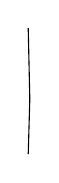
\begin{tikzpicture}\draw (0,0) -- (0.02,0.7) -- (0,1.6);\end{tikzpicture}}}}
\uline{Proposition}\handwritten{5.1.} Le foncteur $\mathbb{M}\handwritten{\longmapsto}V\otimes_{\underline{Z}_p}W$ est une équivalence de la catégorie des faisceaux $p$-adiques constructibles\handwritten{\,}sur $k$ vers la sous-catégorie pleine de la catégorie des F-cristaux \unsure{sur|sar} $k$, formée des F-cristaux $M$ tels que $F_M : M^{\handwritten{\sigma}}\handwritten{\longrightarrow}M$ soit un \uline{isomorphisme} .

\uline{Corollaire}\handwritten{5.\unsure{2|1}.} Le foncteur précédent induit un foncteur pleinement fidèle (compatible avec les $\otimes$-structures)\inserted{\handwritten{$i$}} de la catégorie des
